\documentclass[a4paper]{article}
\usepackage[spanish]{babel}
\usepackage[utf8]{inputenc}
\usepackage{charter}   % tipografia
\usepackage{graphicx}
%\usepackage{makeidx}
\usepackage{paralist} %itemize inline
\usepackage{amssymb}
\usepackage{algorithm}
\usepackage{algorithmic}

%\usepackage{float}
%\usepackage{amsmath, amsthm, amssymb}
%\usepackage{amsfonts}
%\usepackage{sectsty}
%\usepackage{charter}
%\usepackage{wrapfig}
%\usepackage{listings}
%\lstset{language=C}


\usepackage{color} % para snipets de codigo coloreados
\usepackage{fancybox}  % para el sbox de los snipets de codigo

\definecolor{litegrey}{gray}{0.94}

% \newenvironment{sidebar}{%
% 	\begin{Sbox}\begin{minipage}{.85\textwidth}}%
% 	{\end{minipage}\end{Sbox}%
% 		\begin{center}\setlength{\fboxsep}{6pt}%
% 		\shadowbox{\TheSbox}\end{center}}
% \newenvironment{warning}{%
% 	\begin{Sbox}\begin{minipage}{.85\textwidth}\sffamily\lite\small\RaggedRight}%
% 	{\end{minipage}\end{Sbox}%
% 		\begin{center}\setlength{\fboxsep}{6pt}%
% 		\colorbox{litegrey}{\TheSbox}\end{center}}

\newenvironment{codesnippet}{%
	\begin{Sbox}\begin{minipage}{\textwidth}\sffamily\small}%
	{\end{minipage}\end{Sbox}%
		\begin{center}%
		\vspace{-0.4cm}\colorbox{litegrey}{\TheSbox}\end{center}\vspace{0.3cm}}



\usepackage{fancyhdr}
\pagestyle{fancy}

%\renewcommand{\chaptermark}[1]{\markboth{#1}{}}
\renewcommand{\sectionmark}[1]{\markright{\thesection\ - #1}}

\fancyhf{}

\fancyhead[LO]{Sección \rightmark} % \thesection\ 
\fancyfoot[LO]{\small{Cort\'es Lucas, Zimenspitz Ezequiel, Lamela Emanuel}}
\fancyfoot[RO]{\thepage}
\renewcommand{\headrulewidth}{0.5pt}
\renewcommand{\footrulewidth}{0.5pt}
\setlength{\hoffset}{-0.8in}
\setlength{\textwidth}{16cm}
%\setlength{\hoffset}{-1.1cm}
%\setlength{\textwidth}{16cm}
\setlength{\headsep}{0.5cm}
\setlength{\textheight}{25cm}
\setlength{\voffset}{-0.7in}
\setlength{\headwidth}{\textwidth}
\setlength{\headheight}{13.1pt}

\renewcommand{\baselinestretch}{1.1}  % line spacing


% \setcounter{secnumdepth}{2}
\usepackage{underscore}
\usepackage{caratula}
\usepackage{url}


% ******************************************************** %
%              TEMPLATE DE INFORME ORGA2 v0.1              %
% ******************************************************** %
% ******************************************************** %
%                                                          %
% ALGUNOS PAQUETES REQUERIDOS (EN UBUNTU):                 %
% ========================================
%                                                          %
% texlive-latex-base                                       %
% texlive-latex-recommended                                %
% texlive-fonts-recommended                                %
% texlive-latex-extra?                                     %
% texlive-lang-spanish (en ubuntu 13.10)                   %
% ******************************************************** %



\begin{document}


\thispagestyle{empty}
\materia{M\'etodos Num\'ericos}
\submateria{Primer Cuatrimestre de 2016}
\titulo{Trabajo Práctico II}
\subtitulo{CSI: DC}
\integrante{Cort\'es, Lucas}{302/13}{lucascortes@me.com}
\integrante{Lamela, Emanuel}{021/13}{emanuel93_13@hotmail.com}
\integrante{Zimenspitz, Ezequiel}{155/13}{ezeqzim@gmail.com}

\maketitle
\newpage

\thispagestyle{empty}
\vfill
\begin{abstract}
El contexto de este trabajo es el de Sport Analytics, considerando deportes en el cuál el empate no es un resultado posible. El puntapié inicial del mismo es plantear técnicas de armados de rankings basados en la probabilidad de ganar el próximo encuentro de cada equipo. Nuestro objetivo será entonces elaborar métodos para confeccionar estos rankings y realizar análisis comparativos que permitan determinar el que mejor se asimile a la realidad.
\\
\\
\\
\indent \indent \textbf{Palabras claves} \\
\\
$\circ$ Sport Analytics\\
$\circ$ Colley Matrix Method\\
$\circ$ Eliminaci\'on Gaussiana\\
$\circ$ Factorizaci\'on de Cholesky\\
\end{abstract}


\thispagestyle{empty}
\vspace{3cm}
\tableofcontents
\newpage

%\normalsize
\newpage
\section{Introducci\'on Te\'orica}
"¿Qu\'e equipo/qui\'en crees que gana hoy?", una simple pregunta que es dif\'icil de responder con certeza dada la cantidad de aspectos que ofrecen los deportes en general. Antes de analizar una manera de responder la misma con datos y fundamentos te\'oricos, abocamos en algunos casos en los cuáles esto ser\'ia \'util:

\begin{itemize}
\item \textbf{Inversiones:} Convencer de que fortalecer financieramente a una entidad/un jugador es seguro.
\item \textbf{Puntuaci\'on:} En determinados deportes o contextos, vencer a distintos oponentes no siempre genera la misma cantidad de puntos. Esto ayuda a determinar una valuaci\'on de los mismos.
\item \textbf{Medici\'on:} Podr\'ia aportar m\'etricas internas para determinar c\'omo se encuentra la entidad/el jugador comparativamente con los dem\'as.
\end{itemize}

Proveer metodolog\'ias que incorporen aspectos varios y relevantes de los encuentros es esencial para que incremente su precisión. Dicho esto, el m\'etodo que utilizaremos es el \textbf{\textit{Colley Matrix Method}} \textbf{[1]}.

\subsection{Colley Matrix Method}

Este m\'etodo busca obtener las probabilidades de que cada equipo de una liga gane su pr\'oximo encuentro, teniendo en consideraci\'on el schedule que atraves\'o cada uno de ellos (jugar contra los mejores equipos al inicio no indica que vaya a perder contra los peores en los subsiguietntes partidos), sin importar la diferencia de la cantidad de partidos jugados por cada equipo y solo considerando si el equipo gan\'o o perdi\'o (no la diferencia en puntajes obtenidos en los mismos). Es necesario notar que s\'olo aplica a modelos de competencias que no admiten empate como un resultado posible, como los que analizaremos en este contexto.

Definamos primero el modelo utilizado para el problema. Sea $\Gamma = \{1,2,...,T\}$ el conjunto de participantes de la competencia. Luego, para cada equipo \bm{$i \in \Gamma$} denominamos \bm{$n{_i}$} all n\'umero total de partidos jugados por el equipo $i$, \bm{$w{_i}$} al n\'umero de partidos ganados por el equipo $i$ y, an\'alogamente, \bm{$l{_i}$} a la cantidad de encuentros por el equipo $i$. Por \'ultimo, dados $i, j \in \Gamma$, $i \neq j$, \bm{$n{_i}{_j}$} al n\'umero de enfrentamientos entre $i$ y $j$. Una vez definido esto, a través de una serie de postulados y argumentos matemáticos, el paper \textbf{[1]} plantea que las probabilidades se obtienen como resultado de un sistema de ecuaciones lineales de la forma \bm{$Cr = b$}. \\

Donde:

\begin{itemize}
\item 
$C \in R^{T \times T}, C{_i}{_j} =
\left\{
	\begin{array}{lcc}
		-n{_i}{_j} & si & i \neq j \\
		\\ 2 + n{_i} & si & i = j \\
	\end{array}
\right.$
\item $r \in R^{T}$, donde $r{_i} = $ probabilidad de que el equipo i gane su siguiente partido
\item $b \in R^{T}$, donde $b{_i} = 1 + (w{_i} - l{_i}) / 2$
\end{itemize}

Por lo tanto, lo que se busca despejar son los elementos del vector $r$.

$C$ se denomina la \textbf{matriz de Colley} que particularmente, por lo demostrado en \textbf{[1]}, es \textbf{sim\'etrica} ($A = A{^t}$) y \textbf{definida positiva} (\textcolor{red}{DEFINITION HERE}).

Para resolver este sistema, usaremos dos algoritmos distintos para obtener sistemas de f\'acil resoluci\'on por \textit{back-substitution} y \textit{forward-substitution}. \textit{Eliminaci\'on Gaussiana} y \textit{Factorizaci\'on de Cholesky}.

\subsubsection{Eliminaci\'on Gaussiana}

La eliminaci\'on gaussiana es un algoritmo que transforma un sistema de ecuaciones en un sistema equivalente, con la caracter\'istica de que este nuevo sistema es triangular superior.

Esto se logra a través de operaciones que no alteran el conjunto solución de un sistema:

\begin{itemize}
\item Multiplicar una ecuación por un escalar
\item Intercambiar ecuaciones
\item Sumar a una ecuación con un múltiplo de otra
\end{itemize} 

Luego se resuelve por back-substitution y obtenemos el resultado deseado. Sea $A \in R^{nxn}, n \in N$. El sistema $Ax = b$ se transforma en uno equivalente $Ux = b'$, con $U$ una matriz triangular superior. \\

Los $x{_i}$ se obtienen de la siguiente manera: \\

$x{_i} = (b'{_i} - \sum\limits_{j = i + 1}^n u_{ij}x_{i}) / u_{ii}$ \\

Se puede observar que si $\exists \, i \in \{1, ..., n\} / a_{ii} = 0$ entonces no se puede realizar este procedimiento. De todas formas, en este trabajo podemos asegurar que la eliminaci\'on encuentra la $U$ y m\'as a\'un, el sistema tiene soluci\'on \'unica porque la matriz de Colley es, como se mencion\'o anteriormente, sim\'etrica y definida positiva.

Dentro del contexto de uso del \textbf{CMM}, utilizamos la Eliminaci\'on Gaussiana para obtener los $r_i$.

\subsubsection{Factorizacio\'on de Cholesky}

La factorizaci\'on de Cholesky es un caso particular de una factorizaci\'on LU, con L matriz triangular inferior y U matriz triangular superior. Bajo la hip\'otesis de este trabajo sobre las caracter\'isticas de la matriz de Colley, podemos afirmar que existe una factorizaci\'on de la forma LU de C, tal que $U = L{^t}$. \\

$LL{^t}{_i}{_j} =
\left\{
	\begin{array}{lcc}
		\sqrt{C{_i}{_i} - \sum\limits_{k=1}^{i-1} L{_i}{_k}^2} & si & i = j \\
		\\ \frac{1}{L{_i}{_i}}(C{_i}{_j} - \sum\limits_{k=1}^{i-1} L{_i}{_k}L{^t}{_j}{_k}) & si & i \neq j \\
	\end{array}
\right.$ \\

Luego, el sistema equivalente ser\'a $LL{^t}x = b$, entonces puedo resolver $Ly = b$ por forward-substitution y luego $L{^t}x = y$ para obtener el resultado deseado por back-substitution.

\textcolor{red}{\textbf{TODO: Escribir, no olvidar de mencionar por qu\'e y para que se utiliza.}}
\section{Desarrollo}
El suelo est\'a labrado en cuestiones te\'oricas. En esta secci\'on nos avocaremos en explicar el papel que juega cada m\'etodo y, el proceso completo partiendo de las im\'agenes y concluyendo en su clasificaci\'on.

Vamos a considerar las im\'agenes, siendo $n \in \mathbb{N}$ la cantidad, como $x^{(i)} \in \mathbb{R}^{m}$ con $m = 28 \times 28 = 784$ y $i \in \{1, ..., n\}$. Al conjunto de im\'agenes lo denominamos $I$. Como est\'an en escala de grises, adem\'as se cumple que $x^{(i)}_{j} \in \{0, ..., 255\}$, d\'onde $x^{(i)}_{j}$ es el $j$-esimo elemento de $x_{i}$, $\forall j \in \{1, ..., 784\}$. En t\'erminos coloquiales, una \textit{tira} de 784 valores que est\'an en el rango de 0 a 255. Adicionalmente, el conjunto $C = \{0, ..., 9\}$ es el conjunto de clases/\textit{labels}/\textit{tags}/d\'igitos, seg\'un como los denominemos en cada ocasi\'on particular. Finalmente, por ahora, vamos a considerar una partici\'on de $I = A \cup B$, d\'onde $A$ e $B$ son dijuntos y los mismos tienen las particularidades destacadas en \ref{intro_consideraciones}.

\subsection{Metodolog\'ias de Clasificaci\'on}

\subsubsection{Clasificaci\'on \textit{naive} con kNN}

En una primera aproximaci\'on, \textbf{utilizamos el kNN como m\'etodo de clasificaci\'on a secas}, lo que es decidir a qu\'e d\'igito pertenece cada imagen del conjunto $A$. Tomamos $a \in A$ una tira que buscamos \textit{taggear}.

Recordar que, por c\'omo lo definimos en la \textit{secci\'on \ref{intro_knn}}, el algoritmo requer\'ia \textbf{una funci\'on de distancia $\mathbf{d}$}. Como modelamos con vectores, proponemos la \textbf{\textit{norma 2}}. En otras palabras, siendo $z$ y $x$ dos im\'agenes $d(z,x) = \vert\vert z - x \vert\vert_2^2 = (z - x)^{t}(z - x)$. Notar que en su forma de \textit{producto interno}, el c\'omputo no pierde precisi\'on por ser suma y multiplicaci\'on de n\'umeros entre $0$ y $255$. Adicionalmente, fue elegida por el nivel de precisi\'on que posee (en definitiva, compara una a una cada componente). 

En consecuencia de haber definido una $d$, \textbf{obtenemos el conjunto de \textit{$\mathbf{k}$ vecinos m\'as cercanos}}. Clasificar es f\'acil: se cuentan las etiquetas de cada uno de los $k$ vecinos y la que m\'as se repita, se le asigna a $a$ \footnote{En caso de empate, nos quedamos con el primero que hayamos encontrado que maximice la cantidad de apariciones}.

Desafortunadamente, \textbf{la simplicidad tiene su costo temporal en este caso}. Las im\'agenes tienen $784$ pixels, es decir, cada punto a considerar tiene $784$ componentes. Calcular la distancia de un punto de esta dimensi\'on contra \textit{$\vert B \vert$} (el tamaño de $B$) de la misma dimensi\'on suena a mucho trabajo y \textit{lo es}. Aqu\'i es d\'onde cobran valor \textbf{PCA} y \textbf{PLS-DA}.

Ambos tienen la misma idea, obtener una matriz que realice un cambio de base tal que permita quedarnos con s\'olo una \textit{porci\'on}, la de mayor contenido de informaci\'on, de la misma. Aunque por s\'i solos, no son m\'etodos de categorizaci\'on. Por ende, \textbf{estar\'an involucrados como \textit{preprocesadores} de la informaci\'on a ser servida al \textit{kNN}} (reducir las dimensiones a considerar previo a aplicar \textit{kNN}).

\subsubsection{Reducci\'on de dimensi\'on \textit{no} supervisada con \textit{PCA}}

Siguiendo la l\'inea de \textbf{PCA} (\ref{intro_PCA}), buscamos $P$ conformado por las \textit{\textbf{Componentes Principales}} que son los autovectores de $M_{X}$. Inmediatamente surge una imposici\'on en costo de c\'omputo muy elevada: Dado que $M_{X} \in \mathbb{R}^{784 \times 784}$ es sim\'etrica, posee \textit{rango completo} de autovectores. Calcular los $784$ autovectores es pesado, y ,a\'un provisto de ellos, multiplicar \textit{todas} las im\'agenes contra la matriz generada tambi\'en lo es. Esto es bloqueante, lo que busc\'abamos era \textit{reducir} el problema en dimensi\'on para alivianar el costo de c\'omputo.

Provisto de $\alpha \in \mathbb{N}$, y $n_{iter} \in \mathbb{N}$, buscamos generar la transformaci\'on $P \in R^{\alpha \times 784}$ tal que contenga $\alpha$ \textbf{\textit{Componentes Principales}} como filas.
Como dichas componentes son los autovectores, buscamos $\alpha$ autovalores y autovectores de la matriz de covarianzas $M_{X}$. Pero al tomar un n\'umero menor de componentes, se pierde informaci\'on. Por eso mismo, decidimos \textbf{buscar las que maximicen la varianza}, son las que m\'as informaci\'on poseen en el espacio de informaci\'on transformado. Recordando el fundamento del m\'etodo planteado en la secci\'on anterior, buscabamos los autovectores de $M_{X}$ dado que la diagonalizaban. Al estar diagonalizada, los autovalores son los elementos de la diagonal, que a su vez son las varianzas de las variables en \textit{nuevo espacio de datos}. Obtener los de mayor m\'odulo nos aporta la mayor cantidad de informaci\'on posible. Para esto aplica el \textbf{M\'etodo de la Potencia} (explicado en \ref{desarrollo_metodo-potencia}), iterando tantas veces como el $n_{iter}$ provisto, combinado con \textbf{Deflaci\'on} (desarrollado en \ref{desarrollo_deflacion}). Repetimos $\alpha$ veces un paso $i$, con $B^0 = M_{X}$, de: obtener $\lambda_{i}$, el $i$-\'esimo autovalor ordenas por m\'odulo, asociado a $v_{i}$, calcular $B^{i + 1} = B^{i} - \lambda_{i}v_{i}v_{i}^{t}$ y comenzar el paso $i+1$.

Antes de continuar, los algoritmos de generaci\'on de autovectores tienen condiciones sobre los cu\'ales funcionan.

Para el caso de m\'etodo de la potencia:

\begin{itemize}
\item \textcolor{red}{// TODO: Agregar}
\item Como $M_{X}$ es sim\'etrica, tiene todos los autovalores reales.
\end{itemize}

Los requerimientos de deflaci\'on se cumplen dado que:

\begin{itemize}
\item Al ser $M_{X}$ sim\'etrica, sus autovectores generan una \textbf{base ortonormal}.
\end{itemize}

Con lo cu\'al nos quedamos con una matriz $P$ que posee, por filas, los $\alpha$ autovectores de $M_{X}$ que mayor informaci\'on almacenan. El siguiente paso es aplicar el \textit{cambio de base} a cada muestra $z \in Z$ y a $y$: $Py = \hat{y} \in \mathbb{R}^{\alpha}$ y $\hat{z} = Pz \in \mathbb{R}^{\alpha}$, obteniendo sus correspondientes \textit{\textbf{Transformaciones Caracter\'isticas}}. A dicha transformaci\'on la denominamos $\mathbf{tc_{PCA}}$.

\subsubsection{Reducci\'on de dimensi\'on supervisada con \textit{PLS-DA}} \label{desarrollo_PLSDA}

Presentamos un \textit{pseudo-c\'odigo} del procedimiento para luego explicar las decisiones involucradas y las condiciones correspondientes que se deben dar para su correctitud: \\

\begin{algorithm}
\begin{algorithmic}[1]
\FOR {$i \leftarrow [1..\gamma]$}
\STATE {$M_{i} \leftarrow X^{t}YY^{t}X$}
\STATE {$w_{i} \leftarrow$ autovector asociado al mayor autovalor de $M_{i}$} \COMMENT {Deber\'ia estar normalizado, si no, normalizar}
\STATE {$t_{i} \leftarrow Xw_{i}$}
\STATE {Normalizar $t_{i}$}
\STATE {$X \leftarrow X - t_{i}t_{i}^{t}X$}
\STATE {$Y \leftarrow Y - t_{i}t_{i}^{t}Y$}
\ENDFOR
\RETURN {$w_{i}$ para cada $i \leftarrow [1..\gamma]$}
\end{algorithmic}
\caption{PLS($X, Y, \gamma$)}
\end{algorithm}

El algoritmo recibe $X \in R^{n \times 784}$, la matriz de imagenes centralizadas por la media, e $Y$ un vector que \textit{mapea} cada posici\'on con la etiqueta de la im\'agen que se encuentra en la susodicha posici\'on en $X$. Dadas estas construcciones, buscamos ir obteniendo iterativamente los \textbf{autovectores dominantes} $w_{i}$ (autovectores cuyos autovalores sean dominantes en el paso $i$) sobre la matriz $M_{i}$. Notemos que $M_{i}$ es sim\'etrica en todos los pasos: siendo $X = X_{i}$, $Y = Y_{i}$ las matrices iniciales en el paso $i$, vemos que $M_{i}^{t} = (X^{t}YY^{t}X)^{t} = (Y^{t}X)^{t}(X^{t}Y)^{t} = X^{t}(Y^{t})^{t}Y^{t}(X^{t})^{t} = X^{t}YY^{t}X = M_{i}$. Como, por lo desarrollado en \ref{intro_PLSDA}, requerimos $w_{i}$ autovector dominante, utilizamos el \textbf{M\'etodo de la Potencia} (\ref{desarrollo_metodo-potencia}) para extraerlo. El vector resultado se encuentra normalizado, por ende podemos evitar el paso de normalizaci\'on siguiente a su obtenci\'on. Para finalizar la iteraci\'on, en base a $w_{i}$, $X_{i}$ e $Y_{i}$, calcular $t_{i}$ como $Xw_{i}$ para realizar el c\'omputo de $X_{i+1}$ e $Y_{i+1}$.

Las $\gamma$ repeticiones de estos calculos nos otorga $w_{1}$, ..., $w_{\gamma}$ y los utilizamos para obtener la \textbf{Transformaci\'on Caracter\'istica} de una im\'agen $x_{i}$ como $\mathbf{tc_{PLS}(x_{i})} = (w_{1}^{t}x_{i}, ..., w_{\gamma}x_{i}) \in R_{\gamma}$.

\textbf{Con este planteo, tenemos un PLS tracicional}. \textbf{La extensi\'on a PLS-DA la hacemos tomando la $\mathbf{Y}$ como una matriz que centraliza}, como a $X$, \textbf{a una matriz que tiene un $1$ en la posici\'on $(i, j)$ si la imagen $i$ tiene etiqueta $j$\footnote{Indexando desde 1} o $(-1)$ en caso contrario}.

\subsubsection{Clasificaci\'on inteligente: \textit{Transformaci\'on} + \textit{kNN}}

Tanto \textit{PCA} como \textit{PLS-DA} nos facilitan una \textit{transformaci\'on caracter\'istica} que reduce la dimensi\'on de las im\'agenes. Pero \textbf{por s\'i mismos no son \textit{clasificadores}}. Que la dimensi\'on de las im\'agenes se encuentre reducida, abre la posibilidad de utilizar el \textit{kNN} y que su ejecuci\'on se complete en tiempos razonables.

Por lo tanto, \textbf{el algoritmo completo de clasificaci\'on}, sobre una im\'agen particular $y \in Y$ a clasificar, se compone de tomar una $\mathbf{tc_{m}}$, la transformaci\'on caracter\'istica de \textit{PCA} o \textit{PLS-DA}, obtener $tc_{m}(y)$ y $tc_{m}(z_{i})$, con $z_{i} \in Z$, y finalmente utilizar el criterio de clasificaci\'on provisto por \textit{kNN}.

\subsection{Estrategias de medici\'on}

\subsubsection{Evaluaci\'on robusta con \textit{K-fold cross validation}}

\textcolor{red}{// TODO: Fill}

\subsubsection{M\'etricas de calidad}

Finalmente, se desarrollaron algunas m\'etricas para medir qu\'e tan buenas son las decisiones tomadas por el clasificador: \\

* \underline{\textbf{Precision:}} Es una \textbf{medida de cu\'antos aciertos relativos tiene un clasificador dentro de una clase particular}. Es decir, dada una clase $i$, la precision de dicha clase es $tp_{i} / (tp_{i} + fp_{i})$.

En la anterior f\'ormula, $tp_{i}$ son los \textit{verdaderos positivos} de la clase $i$. Es decir, muestras que realmente pertenec\'ian a la clase $i$ y fueron exitosamente identificadas como tales. En contraposici\'on, $fp_{i}$ son los \textit{falsos positivos} de la clase $i$. Son aquellas muestras que fueron identificadas como pertenecientes a la clase $i$ cuando realmente no lo eran.

Luego, la \textit{precision} en el caso de un clasificador de muchas clases, se define como \textbf{el promedio de las precision para cada una de las clases}. \\

* \underline{\textbf{Recall:}} Es una \textbf{medida de que tan bueno es un clasificador para, dada una clase particular, identificar correctamente a los pertenecientes a esa clase}. Dada una clase $i$, el recall de dicha clase es $tp_{i} / (tp_{i} + fn_{i})$.

En la anterior f\'ormula, $fn_{i}$ son los \textit{falsos negativos} de la clase $i$. Es decir, muestras que pertenec\'ian a la clase $i$ pero que fueron identificadas con otra clase.

Luego, el \textit{recall} en el caso de un clasificador de muchas clases, se define como \textbf{el promedio del recall para cada una de las clases}. \\

* \underline{\textbf{F1-Score:}} Dado que precision y recall son dos medidas importantes que no necesariamente tienen la misma calidad para un mismo clasificador, se define esta m\'etrica para \textbf{medir un compromiso entre ambas}. Se define como $2 * precision * recall / (precision + recall)$.

\subsection{Algoritmos de Utilidad}

\subsubsection{M\'etodo de la Potencia}\label{desarrollo_metodo-potencia}

Tenemos una necesidad de encontrar \textit{autovalores} con sus \textit{autovectores asociados}. Para esto utilizamos el \textbf{M\'etodo de la Potencia}. Sea $B^{n \times n}$ la matriz de entrada.

\begin{algorithm}
\begin{algorithmic}[1]
\STATE {$v \leftarrow x_{0}$}
\WHILE {No se cumpla la condici\'on de finalizaci\'on}
\STATE {$v \leftarrow Bv$}
\STATE {Normalizar $v$}
\ENDWHILE
\STATE {$\lambda \leftarrow v^{t}Bv$}
\RETURN {$\lambda, v$}
\end{algorithmic}
\caption{M\'etodo de la Potencia($B, x_{0}$, condici\'on de finalizaci\'on)}
\end{algorithm}

Este m\'etodo busca un autovector $v_{1} \in \mathbb{R}^{m}$ tal que $\vert\vert v \vert\vert_{2} = 1$ aproximando el pasado como par\'ametro iterativamente, con la particularidad de que se corresponde con el autovalor $\lambda_{1} \in \mathbb{R}$ de manera que $\lambda_{1} > \lambda_{i}$ autovalor con $i \neq 1$. Una condici\'on para que converja a este vector es \textcolor{red}{TODO}, notar que para dimensiones grandes, la probabilidad de elegir un vector inicial al azar es pr\'acticamente nula, de modo que el $x_{0}$ es elegido en forma aleatoria. La otra condici\'on es que $B$ tenga todos los autovalores reales. Veremos como ambas condiciones se cumplen para las matrices a las cu\'ales son aplicadas.

\subsubsection{Deflaci\'on}\label{desarrollo_deflacion}

Este algoritmo soslayar\'a un esquema iterativo en el cu\'al uno puede obtener autovalores y autovectores.

Sea $B \in R^{n \times n}$ una matriz que posee autovalores distintos $\lambda_{1}, ..., \lambda_{n}$ con autovectores $v_{1}, ..., v_{n}$ asociados tales que $\vert \lambda_{1} \vert > ... > \vert \lambda_{n} \vert$, en otras palabras poder ordenarlos por m\'odulo. Adem\'as se pide que los autovectores generen una base ortonormal. \textcolor{red}{// TODO: Ver por qu\'e no hace falta que los autovalores no sean distinos} Veamos entonces que: \\

$(B - \lambda_{1}v_{1}v_{1}^{t})v_{1} = Bv_{1} - \lambda_{1}v_{1}(v_{1}^{t}v_{1}) = \lambda_{1}v_{1} - \lambda_{1}v_{1} = 0v_{1}$

$(B - \lambda_{1}v_{1}v_{1}^{t})v_{i} = Bv_{i} - \lambda_{1}v_{1}(v_{1}^{t}v_{i}) = \lambda_{i}v_{i}$ \\

Por lo tanto, la matriz $B - \lambda_{1}v_{1}v_{1}^{t}$ posee autovalores $0, \lambda_{2}, ..., \lambda_{n}$ asociados a $v_{1}, ..., v_{n}$ de tal forma que puedo repetir el proceso obteniendo $\lambda_{2}$ y $v_{2}$. Este algoritmo se acopla muy bien con el M\'etodo de la potencia puesto que el susodicho extrae el autovalor dominante y su correspondiente autovector, con lo cu\'al es perfecto para una combinaci\'on de ambos.
\section{Resultados y discusi\'on}
\subsection{Analisis Previo: Alfa y Gama}
El uso de los m\'etodos de PCA y PLS-DA se funda en reducir la dimensi\'on de los datos a clasificar. La idea es capturar la mayor cantidad de informaci\'on, dejando de lado las componentes que en determinado momento dejen de ofrecernos datos relevantes.

Para esto proponemos el siguiente m\'etodo: Tomamos toda la base de entrenamiento, dejando vac\'ia la base de test, y calculamos los 784 autovalores para ambos m\'etodos. Sea $\lambda_{PCA}$ la suma de los autovalores obtenidos por PCA y $\lambda_{PLS-DA}$ la suma de los obtenidos por PLS-DA.

En el caso de PCA, como siempre calculamos los autovalores de la matriz de covarianzas, se cumple que la suma de los autovalores es igual a la suma de las varianzas, es decir, a la suma de la diagonal de la matriz de covarianzas. \textcolor{red}{BUSCAR DEMO O DEJAR ASI}. Entonces podemos decir que $\lambda_{PCA}^{i} / \lambda_{PCA}$ representa el porcentaje de varianza que absorbe el autovalor $i$-\'esimo.

Si acumulamos las varianzas que absorbe cada vector, se genera el gr\'afico \ref{accum_var_PCA}

\begin{figure}[h!]
  \begin{center}
	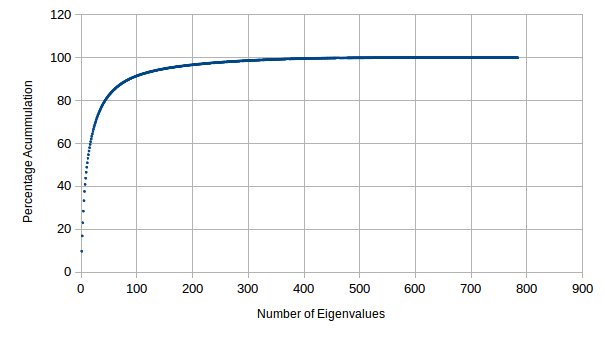
\includegraphics[scale=1]{exp4/PCA-percentage.png}
	\caption{Porcentaje de varianzas acumuladas: PCA}
	\label{accum_var_PCA}
  \end{center}
\end{figure}

Puede verse que el primer autovector se lleva el 10\% de la varianza, el segundo casi un 7\%. Pero es m\'as interesante cuando se llega a tomar 50 autovalores, en esta caso, ya se tom\'o cerca de 83\% de la informaci\'on. Con lo cual, podr\'iamos pensar los dem\'as autovalores no son tan significativos \footnote{El 90\% se alcanza con 86 autovalores. El 99\% con 330}.

Para el caso de PLS-DA, no se calculan los autovalores de la misma matriz en cada paso, haciendo que el an\'alisis anterior no sea del todo directo. Notemos que el autovalor obtenido en cada paso, si bien es de una matriz diferente, tiene la idea de maximimar las varianzas y minimizar las covarianzas de la uni\'on entre las im\'agenes y sus etiquetas. Entonces decidimos aplicar el mismo procedimiento, obteniendo el gr\'afico \ref{accum_var_PLSDA}

\begin{figure}[h!]
  \begin{center}
	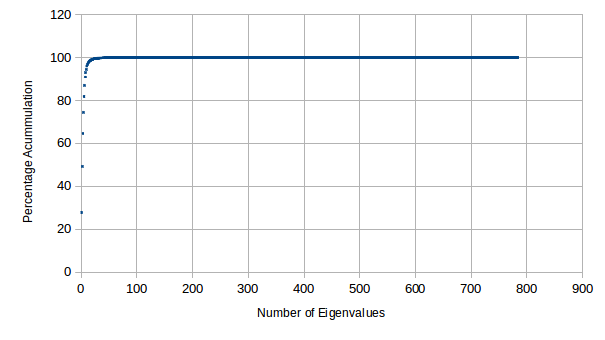
\includegraphics[scale=1]{exp4/PLSDA-percentage.png}
	\caption{Porcentaje de varianzas acumuladas: PLS-DA}
	\label{accum_var_PLSDA}
  \end{center}
\end{figure}

En este se ve que ya el primer autovector, captura cerca del 30\% de la informaci\'on. Junto al segundo, consumen casi el 50\%. Esto indica que tener en cuenta la etiqueta a la hora de intentar reducir la dimensi\'on de los datos puede ser muy \'util. De hecho, con 8 autovalores se captura el 90\% y con 18 ya el 99\%

Los subsiguientes an\'alisis cualitativos fueron realizados bajo estas conclusiones. Es decir, no consideramos tomar $\alpha$ mayor a 300 ni $\gamma$ mayor a 20.

\newpage
\subsection{El nuevo espacio}\label{resultados_new-space}
Cada autovector que buscamos, proporciona nueva informaci\'on para nuestro an\'alisis. En esta secci\'on vamos a intentar ver cu\'al es esta informaci\'on, es decir, qu\'e es lo que nos est\'a diciendo cada autovector.

Vamos a tomar \'unicamente los primeros 3 autovectores obtenidos por cada m\'etodo, porque no se pueden graficar puntos en m\'as de 3 dimensiones.

\begin{table}[h!]
\begin{center}
\begin{tabular}{|c|c|c|}
	\hline
	\# & PCA & PLS-DA \\
	\hline
	Primer Autod\'igito &
	
\includegraphics[scale=4.00]{exp3/PCA-1} &
	
\includegraphics[scale=4.00]{exp3/PLS-1} \\
	\hline
	Segundo Autod\'igito &
	
\includegraphics[scale=4.00]{exp3/PCA-2} &
	
\includegraphics[scale=4.00]{exp3/PLS-2} \\
	\hline
	Tercer Autod\'igito &
	
\includegraphics[scale=4.00]{exp3/PCA-3} &
	
\includegraphics[scale=4.00]{exp3/PLS-3} \\
	\hline
\end{tabular}
\end{center}
\caption{Primeros autod\'igitos de los m\'etodos}
\end{table}

La tabla anterior muestra los 3 primeros autod\'igitos obtenidos para cada m\'etodo. Para obtener cada uno, se obtuvo el autovector asociado a cada uno de los primeros 3 autovalores, que est\'an normalizados. Se los convierte a base 0 - 1 \footnote{$(x^{i} - x_{min}) / (x_{max} - x_{min})$, con $x_{min}$ el m\'inimo valor encontrado en x y $x_{max}$ el m\'aximo, $x^{i}$ el $i$-\'esimo elemento de x} y se los multiplica por 255. As\'i obtenemos una matriz con valores entre 0 y 255 que representa una imagen, en particular la de los autod\'igitos.

\textbf{Hip\'otesis:} Dada la forma del primer autod\'igito, el primer autovector no admite confusi\'on entre los d\'igitos 0 y 1.

Para ver si esto vale, vamos a mostrar el extracto pertinente de las matrices de confusi\'on obtenidas para PCA y PLS-DA respectivamente:

\begin{table}[h!]
\begin{subtable}{.5\linewidth}
\begin{tabular}{|c|c|c|}
	\hline
	Actual\textbackslash Predicted & 0 & 1 \\
	\hline
	0 & 3009 & 0 \\
	\hline
	1 & 0 & 4091 \\
	\hline
\end{tabular}
\end{subtable}
\begin{subtable}{.5\linewidth}
\begin{tabular}{|c|c|c|}
	\hline
	Actual\textbackslash Predicted & 0 & 1 \\
	\hline
	0 & 3213 & 0 \\
	\hline
	1 & 0 & 3924 \\
	\hline
\end{tabular}
\end{subtable}
\end{table}

Se puede apreciar que la confusi\'on entre ambos d\'igitos es nula, el resto de la matriz no aporta grandes resultados, a excepci\'on que para el d\'igito 1:

Para PCA:

\begin{table}[h!]
\begin{tabular}{|c|c|c|c|c|c|c|c|c|c|c|}
	\hline
	Actual\textbackslash Predicted & 0 & 1 & 2 & 3 & 4 & 5 & 6 & 7 & 8 & 9 \\
	\hline
	1 & 0 & 3649 & 57 & 44 & 151 & 45 & 61 & 374 & 65 & 238 \\
	\hline
\end{tabular}
\end{table}

Para PLS-DA

\begin{table}[h!]
\begin{tabular}{|c|c|c|c|c|c|c|c|c|c|c|}
	\hline
	Actual\textbackslash Predicted & 0 & 1 & 2 & 3 & 4 & 5 & 6 & 7 & 8 & 9 \\
	\hline
	1 & 0 & 3924 & 8 & 25 & 91 & 7 & 7 & 421 & 24 & 177 \\
	\hline
\end{tabular}
\end{table}

Muestran que cuando la imagen a etiquetar es un 1, en la mayor\'ia de los casos va a acertar, pero si no lo hace, es m\'as probable que lo confunda con un 7 o con un 9, lo cual tiene sentido ya que los d\'igitos se parecen en su forma.

Es interesante entonces mostrar como se distribuyen los puntos en el nuevo espacio \footnote{El eje $y$ no es representativo, se tomo para simular $\mathbb{R}^{2}$}.

\begin{figure}[h!]
  \begin{center}
	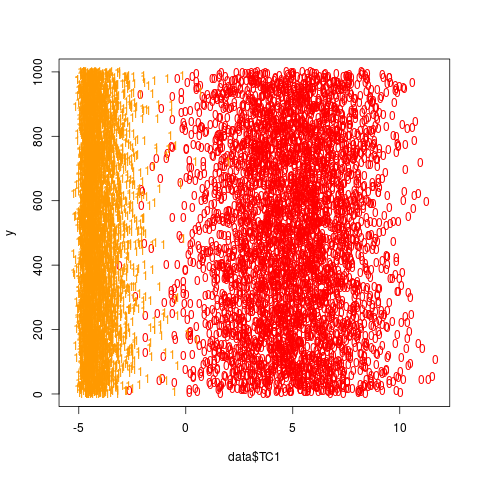
\includegraphics[scale=0.8]{exp5/PCA-1-0vs1}
	\caption{0 VS 1. Puntos en el nuevo espacio PCA}
  \end{center}
\end{figure}

\newpage

\begin{figure}[h!]
  \begin{center}
	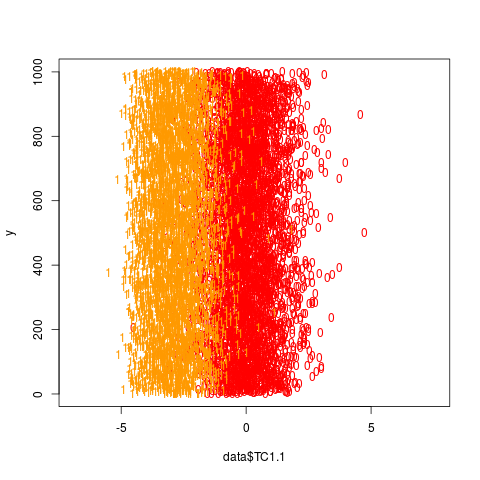
\includegraphics[scale=0.8]{exp5/PLS-1-0vs1}
	\caption{0 VS 1. Puntos en el nuevo espacio PLS-DA}
  \end{center}
\end{figure}

En PCA se ve una clara distancia entre los puntos transformados con etiquetas 0 y 1, guiados por el rasgo distintivo del autod\'igito. En PLS-DA parecer\'ia que se confunden en la frontera, aunque la mayor densidad de puntos est\'a en la media de cada uno, por lo que kNN clasificando un punto sobre la frontera no deber\'ia tener problemas \footnote{No pudimos encontrar una explicaci\'on para este fen\'omeno, creemos que la mayor\'ia de los 1's que se acercan a la media del 0 est\'an en la base de entrenamiento}.


\newpage
\subsection{Análisis de KNN}\label{resultados_knn}
\subsubsection{Costo temporal}

El algoritmo KNN es temporalmente costoso ya que para calcular la distancia entre dos vectores hay que considerar a todas sus coordenadas. Por lo tanto somos muy dependientes del tamaño del vector, que en general al trabajar con imágenes suelen ser bastante grandes.


Para analizar nuestro dataset con KNN utilizamos cross validation con $K = 5$ y $K = 10$.

En la siguiente figura se pueden ver los tiempos de ejecución promedio de las particiones para cada valor de K.

\begin{figure}[h!]
  \begin{center}
	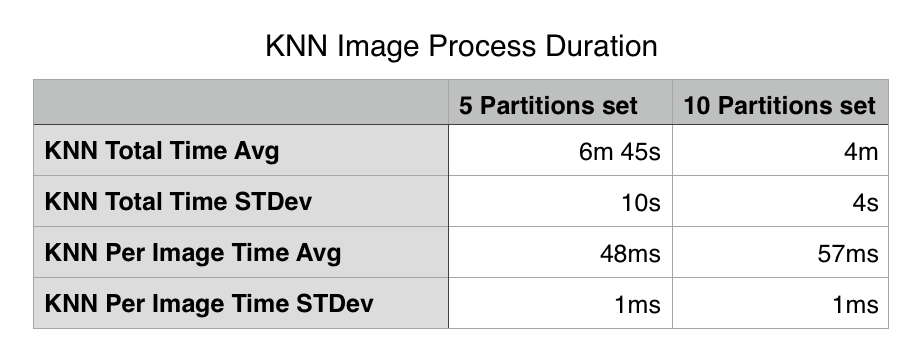
\includegraphics[scale=0.7]{exp1/KNN-Image-Process-Duration.png}
	\caption{KNN Image Process Duration}
%	\label{accum_var_PCA}
  \end{center}
\end{figure}


Para el caso de $K = 5$ obtuvimos que etiquetar una imagen usando KNN tardó en promedio 48ms, que aunque parece poco, al correr todo nuestro set de test de 8400 imágenes se obtuvo un tiempo de ejecución promedio de 6.75 minutos con 10 segundos de desvío estándar. Se puede observar fácilmente que si quisiésemos clasificar un millón de imágenes se tardaría aproximadamente 13 horas.

Por otro lado, vemos que si realizamos 10 particiones a nuestro dataset, el tiempo de procesamiento de cada imagen aumenta de 48ms a 57ms. Esto se debe a que con 10 particiones se debe buscar el vecino más cercano entre más imágenes.

Debemos aclarar también que el costo temporal de variar la cantidad de vecinos de KNN es lineal y por lo tanto esto no tiene una influencia significativa en el tiempo de ejecución. En consecuencia decidimos analizar la calidad de los resultados de KNN disminuyendo la importancia del costo de agregar más vecinos.

\subsubsection{Calidad del algoritmo}

Analizamos la calidad de KNN (con K = 5) calculando su Hit Rate, Precision, Recall y F1 score. Se pueden observar los resultados en el siguiente gráfico.

\newpage

\begin{figure}[h!]
  \begin{center}
	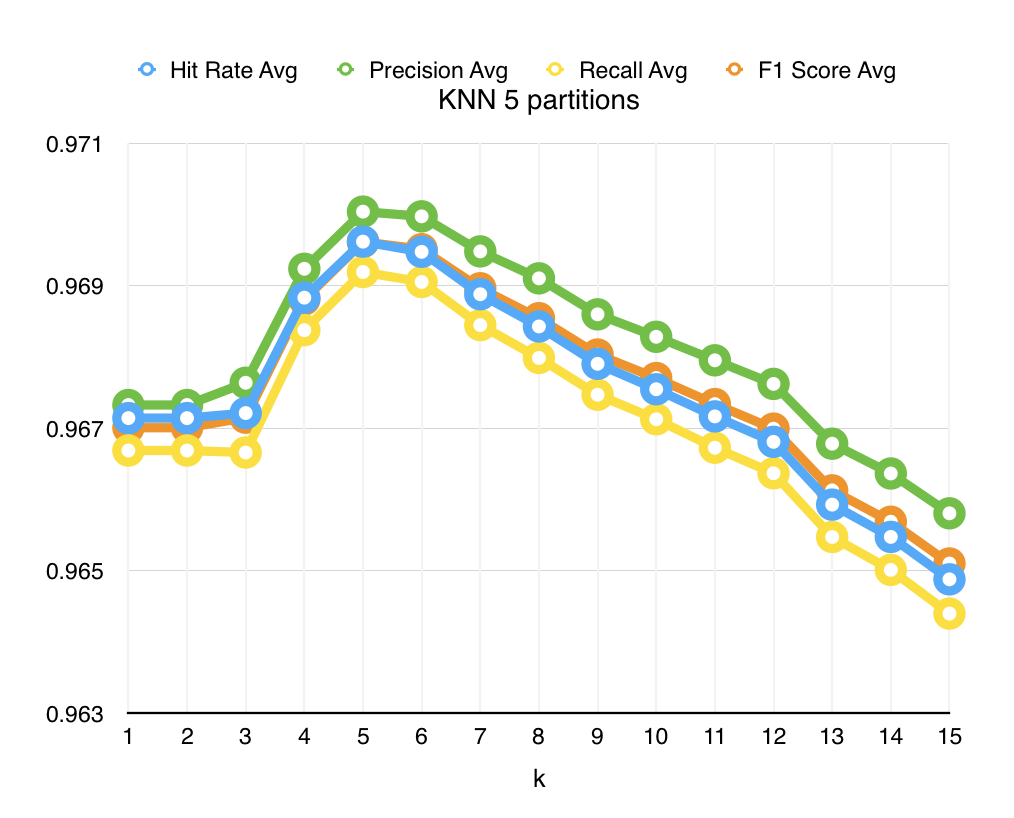
\includegraphics[scale=0.7]{exp1/KNN-5p-Scores.png}
	\caption{KNN quality comparison}
%	\label{accum_var_PCA}
  \end{center}
\end{figure}

Una de las primeras cosas que se pueden observar es que la calidad de los resultados es extremadamente buena. El hit rate promedio para el mejor k es 0.97. Es notable el valor y la similitud entre los resultados de las distintas m\'etricas. Ese rasgo denota una \textit{matriz de confusi\'on} subyacente que es saludable. Dicho fen\'omeno se debe a que: 

\begin{itemize}
\item Por una parte, la \textit{precision} nos indica cu\'antos \textit{aciertos reales} hubo dentro de los \textit{predichos}. (ej: porcentaje de 8's predichos correctamente dentro de todos los clasificados como 8)
\item Por la otra, \textit{recall} otorga el porcentaje de \textit{aciertos} dentro de todos los elementos pertenecientes a una clase. (ej: porcentaje 8's predichos dentros de todos los 8's reales)
\end{itemize}

Al haber obtenido buenos y similares resultados en las susodichas m\'etricas, se habilita un an\'alisis m\'as objetivo del \textit{hit-rate} puesto que suele aplanar s\'intomas negativos ya que es meramente ``adivinados sobre totales''. Esta relaci\'on entre ambas m\'etricas es resumida en el \textit{F1-Score} y  natural que sus valores sean elevados ya que es una relaci\'on entre ambos. Es cierto que hay una preponderancia de \textit{precision} por sobre \textit{recall}, con lo cu\'al uno estar\'ia tentado a decir que es mayormente contundente dentro de sus propias predicciones que en lo que en realidad ocurre. Esta afirmaci\'on es emp\'iricamente cierta, pero de todas formas la diferencia de $\sim$0.005 que presentan no creemos que es suficiente como para ser concluyentes.

Por otro lado también se puede ver que, a partir de k = 5, al aumentar la cantidad de vecinos la calidad de los resultados disminuye. Esto se debe probablemente a que considerar más imágenes comienza a agregar ruido a la medición. Al considerar más vecinos que cada vez se empiezan a parecer menos, es posible que se incorporen un conjunto cada vez mayor de imágenes que pertenecen a otra clase. Así mismo podemos ver que desde 1 vecino hasta 5 la información que aporta agregar más vecinos es valiosa y ayuda mejorar la clasificación.\\

Analizando el hit rate más detalladamente obtenemos el siguiente gráfico donde podemos observar su desvío estándar.

\newpage

\begin{figure}[h!]
  \begin{center}
	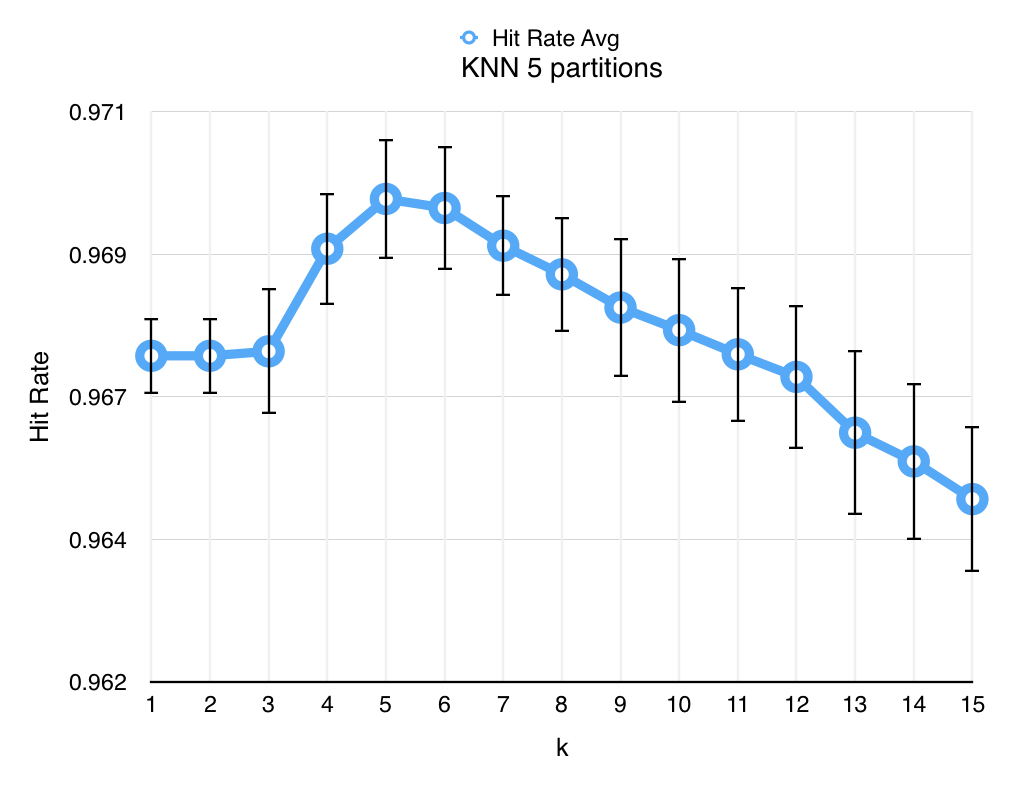
\includegraphics[scale=0.7]{exp1/KNN-5p-Hit-Rate.png}
	\caption{KNN hit rate}
%	\label{accum_var_PCA}
  \end{center}
\end{figure}

Por un lado podemos ver que el desvío estándar es relativamente pequeño. Este desvío representa los diferentes resultados del Hit Rate para cada partición de nuestro data set. Entonces sabemos que todas nuestras particiones tienen un buen resultado y no estamos sesgando nuestro testeo.
Otra cosa interesante que se desprende del gráfico es que los desvíos estándar van aumentando a medida que se incrementa la cantidad de vecinos de KNN. De hecho en el siguiente gráfico podemos ver este incremento.

\begin{figure}[h!]
  \begin{center}
	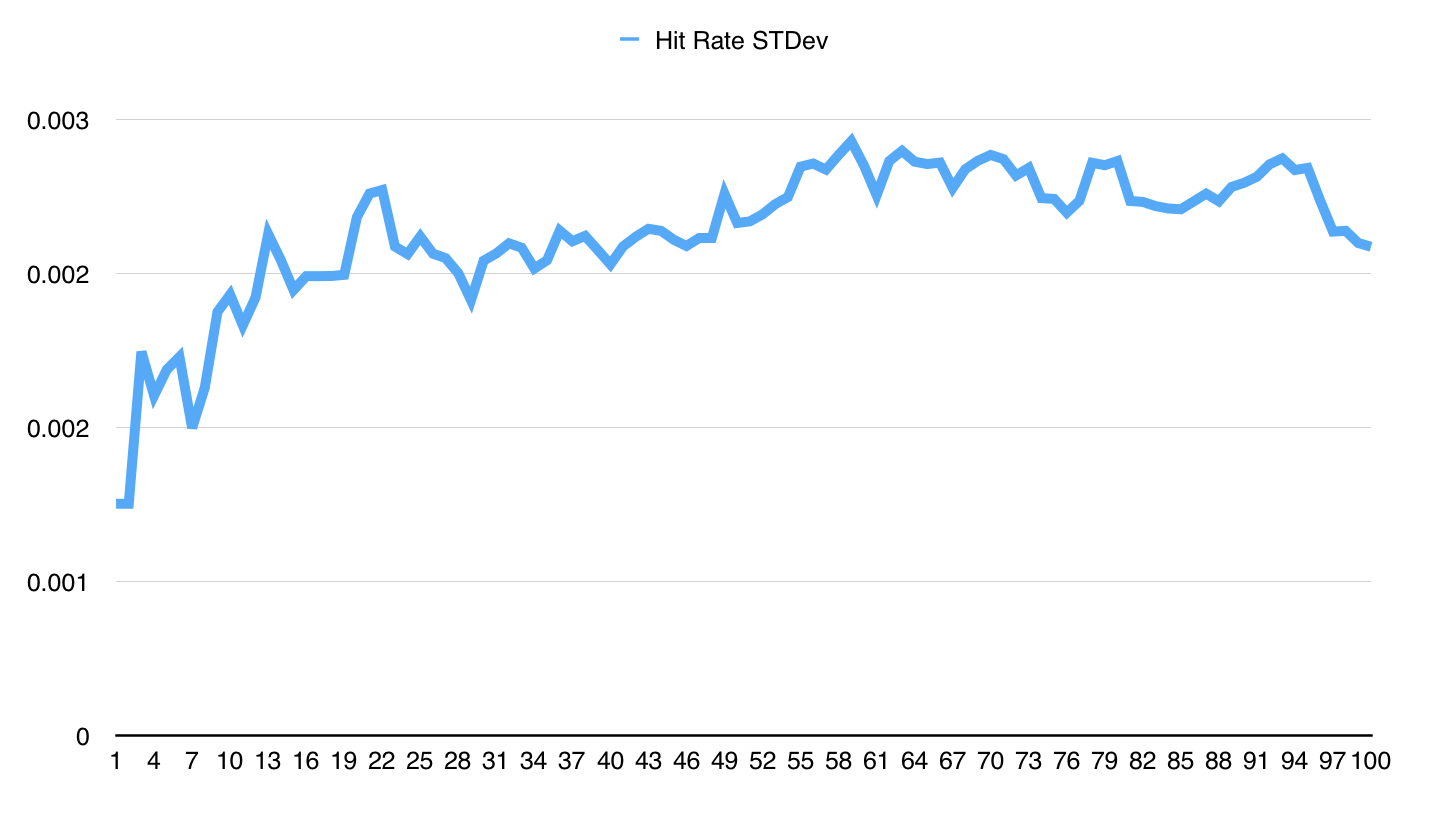
\includegraphics[scale=0.5]{exp1/KNN-5p-Hit-Rate-stdev.png}
	\caption{KNN hit rate standard deviation}
%	\label{accum_var_PCA}
  \end{center}
\end{figure}

Aunque los números se mantienen pequeños, es claro que agregar más vecinos incrementa el ruido y hace divergir más la calidad de los resultados en cada partición.\\

Una vez determinado que k = 5 optimiza la calidad de KNN y además no compromete el tiempo de ejecución, veamos en particular cómo está clasificando a nuestro dataset.


\begin{figure}[h!]
  \begin{center}
	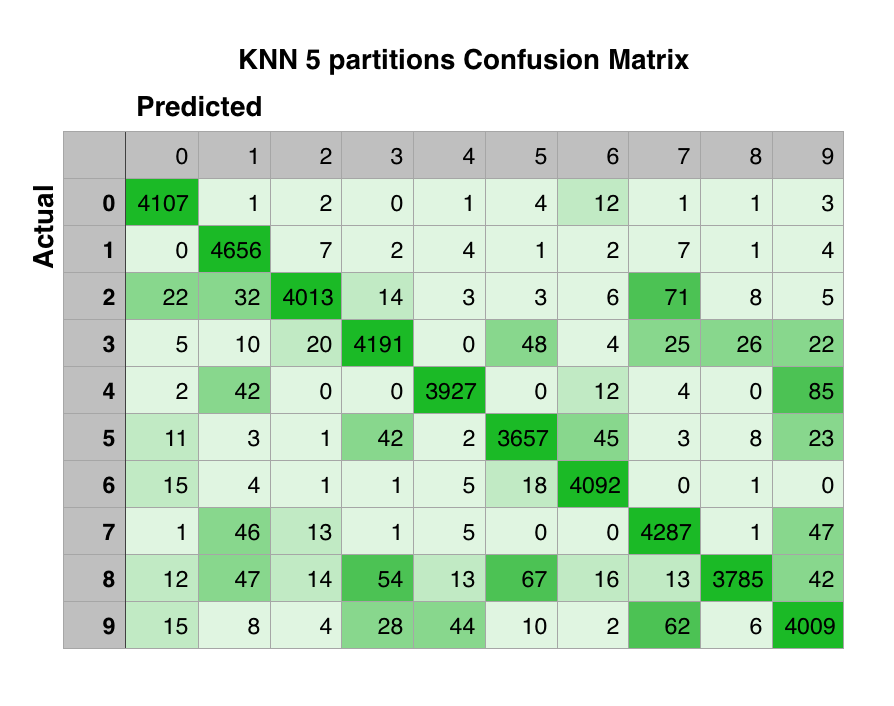
\includegraphics[scale=0.7]{exp1/KNN-5p-Confusion.png}
	\caption{KNN Confusion Matrix}
%	\label{accum_var_PCA}
  \end{center}
\end{figure}

Esta matriz de confusión es la suma de las matrices de confusión de cada una de las 5 particiones del test. Nos muestra claramente en su diagonal las clasificaciones acertadas y en el resto de las posiciones las que no clasificó correctamente. Vemos que los números fuera de la diagonal en general son bajos y que los más altos en general son casos que justifican cierto error. Por ejemplo, hubo setenta y un $2$ que clasificó como $7$ y a su vez hubo cuarenta y seis $7$ que clasificó como $2$. También vemos cierta confusión entre el 4 y 9, 8 y 5, etc. Se puede ver claramente como la matriz de confusi\'on se condice con los datos plasmados en el gr\'afico de las m\'etricas. Esto corrobora que de la diferencia entre \textit{precision} y \textit{recall} no denotaba una inclinaci\'on relevante por una o la otra, por ejemplo, con los d\'igitos 1 y 2: la \textit{precision} para la clase 1 es notoriamente menor que para 2, y lo contrario ocurre con \textit{recall}. El resto tiene mayor equitatividad entre ambas m\'etricas si uno observa con detenimiento. \\ 

Todo este análisis realizado para K = 5 lo hicimos también para K = 10. 

En el siguiente gráfico podemos observar que las medidas de calidad son similares al anterior caso y k = 5 sigue siendo el máximo.\\

\newpage

\begin{figure}[h!]
  \begin{center}
	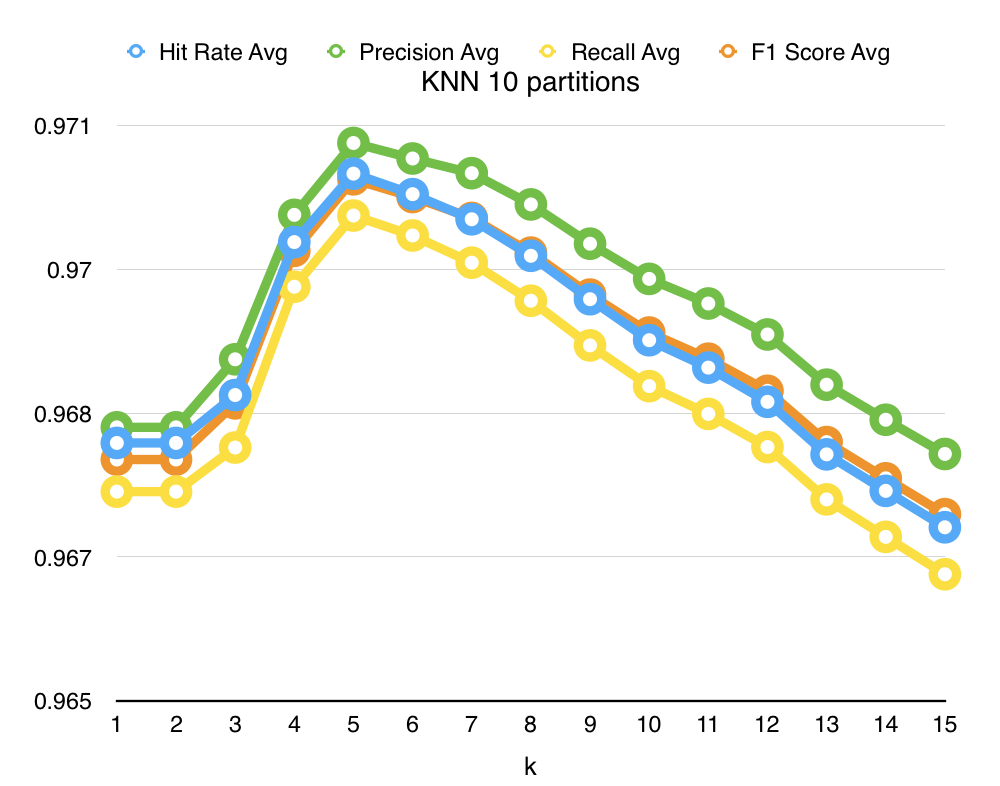
\includegraphics[scale=0.7]{exp1/KNN-10p-Scores.png}
	\caption{KNN Hit Rate (10 partitions)}
%	\label{accum_var_PCA}
  \end{center}
\end{figure}

Comparando los desvíos estándar se puede ver que con 10 particiones el desvío es bastante superior al caso anterior. Esto probablemente se deba a que al haber más particiones de tamaño más pequeño, los casos que la base de entrenamiento no sabe reconocer no estén tan uniformemente distribuidos en esos 10 conjuntos. Un an\'alisis \textit{cuasi} id\'entico de comparaci\'on de m\'etricas hecho con K = 5 puede aplicar para este caso tambi\'en. Lo remarcable es el nivel de consistencia que se mantiene entre los 2 experimentos, lo cu\'al es un argumento a favor en la calidad de las metodolog\'ias de medici\'on planteadas. \\ 

\begin{figure}[h!]
  \begin{center}
	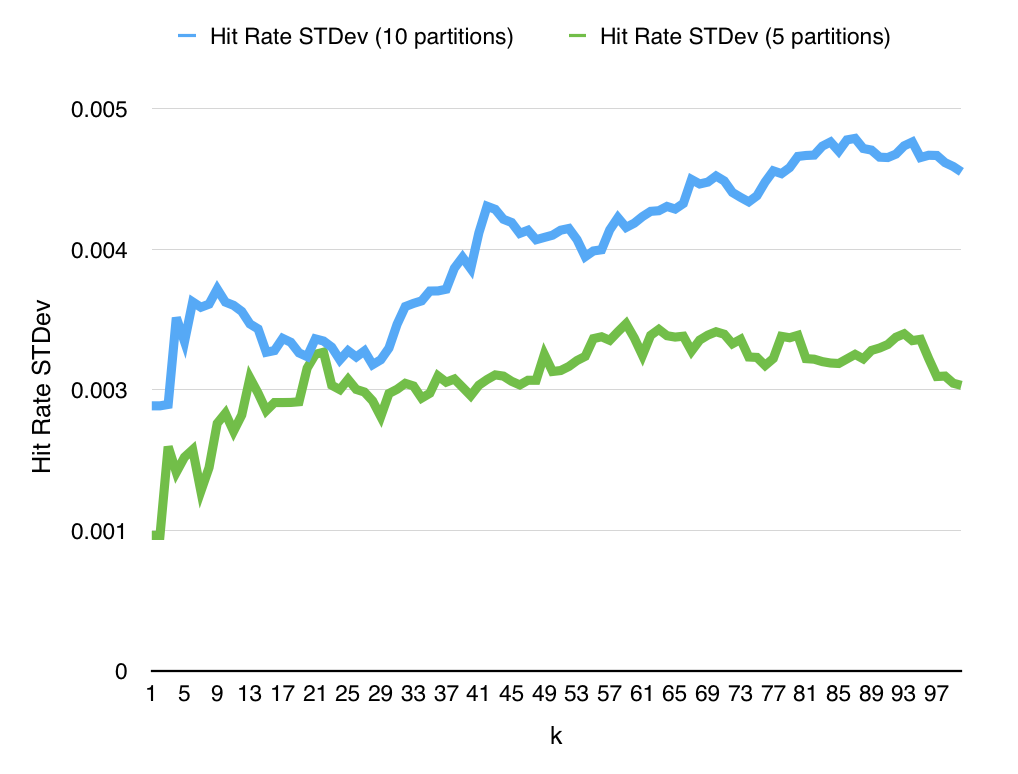
\includegraphics[scale=0.7]{exp1/KNN-Hit-Rate-stdev.png}
	\caption{KNN Hit Rate (10 partitions)}
%	\label{accum_var_PCA}
  \end{center}
\end{figure}

Por último comparamos el hit rate entre los 2 conjuntos de particiones y observamos que el caso de 10 particiones tiene un hit rate ligeramente superior. Esto se debe a que su base de entrenamiento es más grande y puede así reconocer mejor los dígitos.\\

\begin{figure}[h!]
  \begin{center}
	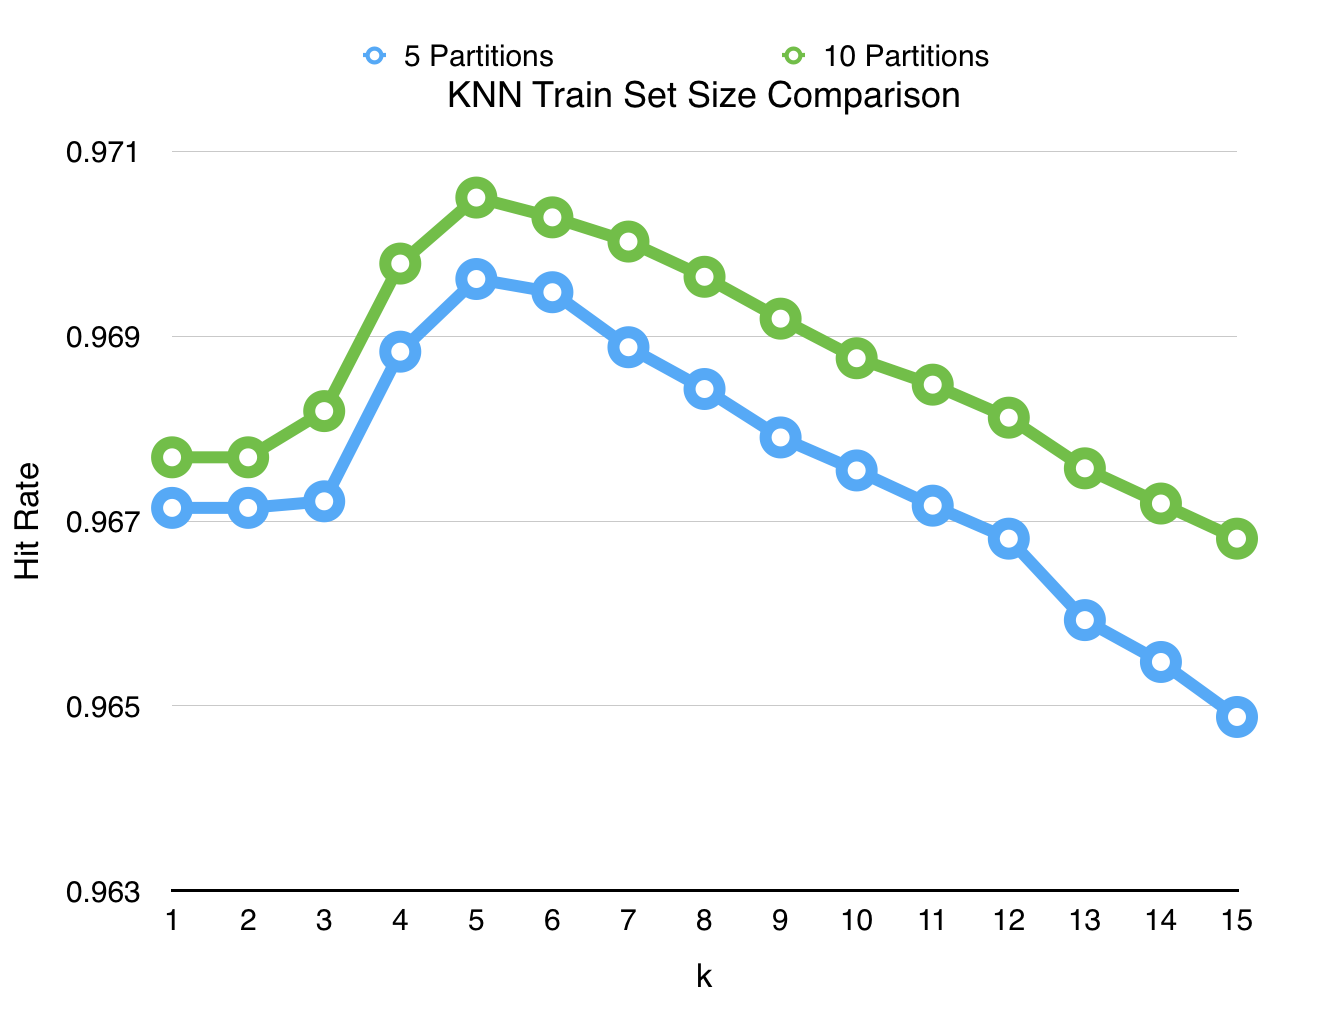
\includegraphics[scale=0.6]{exp1/KNN-Train-Set-Size.png}
	\caption{KNN Hit Rate (10 partitions)}
%	\label{accum_var_PCA}
  \end{center}
\end{figure}





\newpage
\subsection{Análisis de PCA y PLS-DA con kNN}
\subsubsection{Descripción}

En esta sección trataremos de encontrar cuáles son los parámetros que optimizan los resultados de KNN al preprocesar la información usando PCA y PLS-DA. Para esto tendremos en cuenta los tiempos de ejecución de los algoritmos para encontrar la mejor relación entre calidad y costo temporal.



\section{Conclusiones}
\section{Conclusiones}
\section{Referencias}
\textbf{[1]} An\'alisis Num\'erico, p\'agina 491 - Burden \& Faires

%\begin{figure}
%  \begin{center}
%	
\includegraphics[scale=0.66]{imagenes/logouba.jpg}
%	\caption{Descripcion de la figura}
%	\label{nombreparareferenciar}
%  \end{center}
%\end{figure}

%\paragraph{\textbf{Titulo del parrafo} } Bla bla bla bla.
%Esto se muestra en la figura~\ref{nombreparareferenciar}.

%\begin{codesnippet}
%\begin{verbatim}
%
%struct Pepe {
%
%    ...
%
%};
%
%\end{verbatim}
%\end{codesnippet}

%\section{Enunciado y solucion} 
%\input{enunciado}

\end{document}

